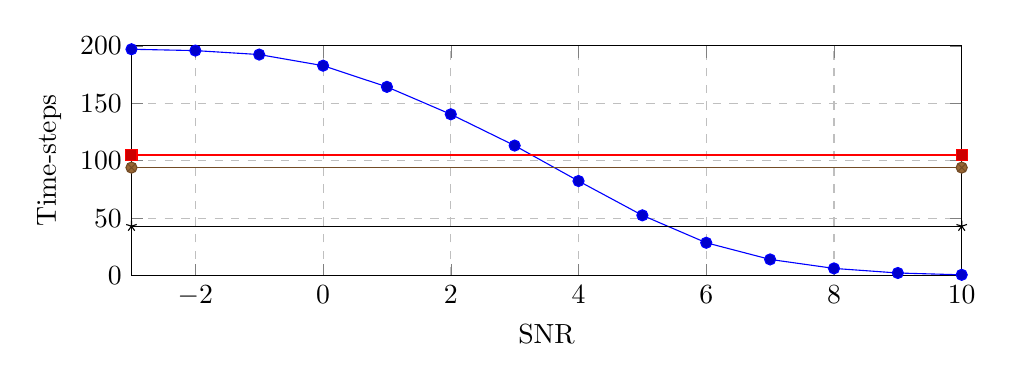
\begin{tikzpicture}

\begin{axis}[
scale=1,
xmin=-3,
xmax=10,
ymin=0,
ymax=200,
ymajorgrids=true,
xmajorgrids=true,
grid style=dashed,
width=\linewidth, height=4.5cm,
xlabel={SNR},
ylabel={Time-steps},
%ylabel shift=-7,
legend cell align={left},
legend pos=north east,
legend style={
	column sep=0mm,
	font=\fontsize{9pt}{9}\selectfont,
},
legend to name=legend-PLatcompSCL,
legend columns=4,
]

%\addplot
%table {
%-3 96.74
%-2 95.27
%-1 91.81
%0 85.23
%1 75.11
%2 62.16
%3 48.16
%4 34.86
%5 23.24
%6 14.11
%7 7.77
%8 3.57
%9 1.37
%10 0.42
%};
%\addlegendentry{GA}

\addplot
table {
-3 197.00
-2 195.83
-1 192.39
0  182.71
1  164.27
2  140.40
3  113.17
4  82.320
5  52.460
6  28.590
7  14.090
8  6.2700
9  2.2800
10 0.6900
};
\addlegendentry{Proposed}

\addplot
table {
-3 105
10 105
};
\addlegendentry{SCL \cite{hashemi2016fast}}

\addplot
table {
-3 94
10 94
};
\addlegendentry{SCL \cite{hashemi2017fast}}

\addplot
table {
-3 43
10 43
};
\addlegendentry{SCL \cite{hanif2018fast}}

\end{axis}
\end{tikzpicture}